\documentclass[a4paper,12pt]{article}
%\usepackage[latin1]{inputenc}
\usepackage[spanish]{babel}
\usepackage{graphicx}
\usepackage{amsmath}
\spanishdecimal{.}
\usepackage{wrapfig}
\setlength{\textheight}{250mm}
\setlength{\textwidth}{165mm}
\setlength{\topmargin}{-15mm}
\setlength{\oddsidemargin}{0pt}
\pagestyle{empty}


\renewcommand{\labelenumi}{\alph{enumi})}

\begin{document}

\def\bm#1{{\mbox{\boldmath $#1$}}}
\def\eqdef{\buildrel \rm def \over =}
\def\signo{\mathop{\rm signo}\nolimits}

\mbox{}\vspace*{-20mm}

{\centering
{\small\sc %Escuela Técnica Superior de Ingenieros de Caminos, Canales y Puertos (Madrid)}\\*[4mm]
Máster Universitario en Ingeniería de Estructuras, Cimentaciones y Materiales}\\*[4mm]
{\Large\bf Método de los Elementos Finitos 25-26}\\*[4mm]
% Puedes cambiar el número de práctica según corresponda
PRÁCTICA 5: Elasticidad lineal 3D (Elementos Isoparamétricos). \\*[4mm]}

% \vspace{4mm}

% ENUNCIADO
\begin{wrapfigure}[16]{r}[5mm]{80mm}
\centering
% IMPORTANTE: Asegúrate de que la imagen esquemática que generamos
% se llame 'escuadra_esquema' y esté en la misma carpeta, o cambia
% el nombre aquí. Se recomienda formato PNG o PDF para LaTeX.
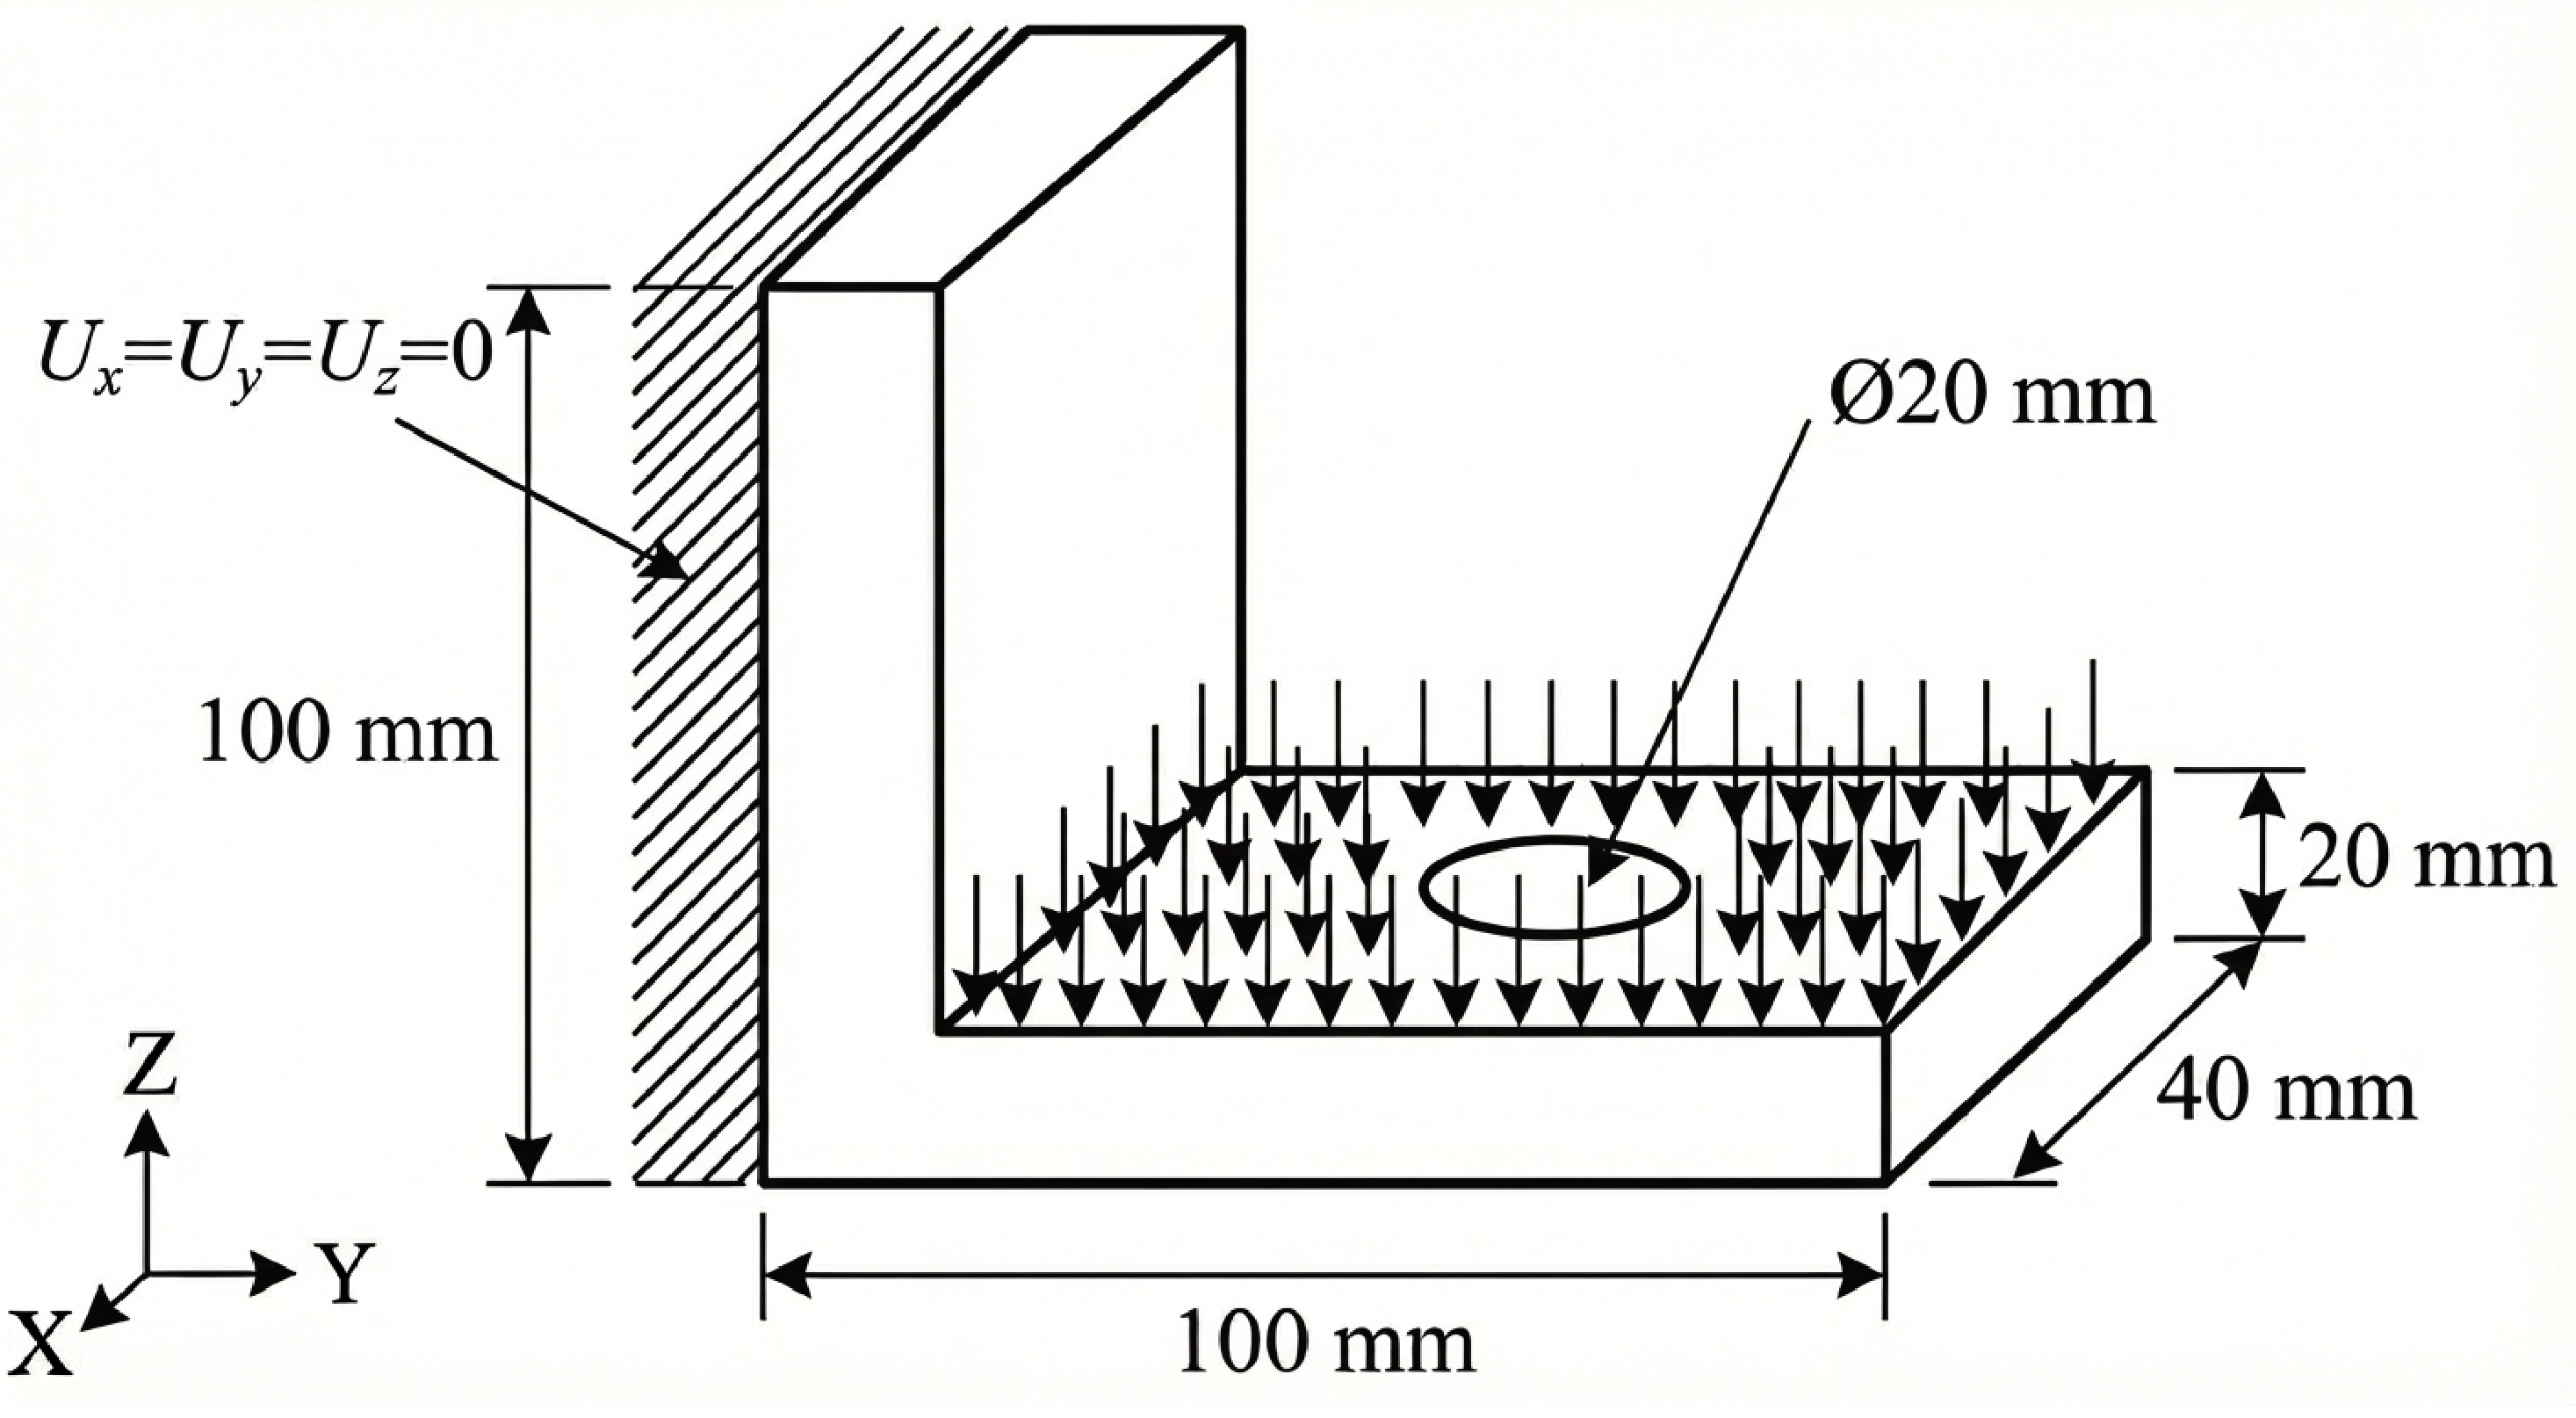
\includegraphics[width=80mm]{escuadra.pdf}
\caption{\small Esquema de geometría, carga y condiciones de contorno.}
\end{wrapfigure}

En esta práctica se analiza el comportamiento mecánico de una escuadra de soporte (L-bracket) con un orificio pasante. Dicho orificio esta centrada en la cara sometida a presión. La pieza está sometida a una carga de presión en una de sus caras y se encuentra empotrada en la cara posterior del brazo vertical.

Se empleará un modelo de elasticidad lineal isótropa 3D para determinar el estado tensional y de deformación de la pieza bajo las cargas indicadas.

Los valores de los distintos parámetros que definen el problema son:

\begin{itemize}
\item \textbf{Material} (Acero):
    \begin{itemize}
    \item $E$: Módulo de Young = $210\,000$ MPa.
    \item $\nu$: Coeficiente de Poisson = 0.3.
    \end{itemize}
\item \textbf{Cargas y Condiciones de Contorno}:
    \begin{itemize}
    \item Empotramiento ($U_x=U_y=U_z=0$) en la cara trasera vertical.
    \item Presión $P = 5$ MPa aplicada verticalmente hacia abajo sobre la cara superior del brazo horizontal.
    \end{itemize}
\end{itemize}

\vspace{5mm}

\textbf{Nota:}

La malla deberá estar formada por elementos finitos tetrahédricos lineales (C3D4). Se sugiere un tamaño de elemento global aproximado de 8 mm.

\vspace{5mm}

\textbf{Se pide:}

Una vez realizado el análisis, obtener y presentar los siguientes resultados en el visualizador:

\begin{enumerate}
    \item Comprobar la deformada de la pieza para verificar que las condiciones de contorno y el sentido de la carga se han aplicado correctamente.
    \item Obtener el contorno de tensiones de Von Mises (S, Mises). Identificar el valor máximo y localizar en qué zonas de la pieza se produce dicho máximo (concentración de tensiones). Solución: 178.3 MPa
    \item Obtener el contorno de desplazamientos verticales (U3) e indicar el valor del desplazamiento máximo (en magnitud) en el extremo libre de la escuadra. Solución: 0.23 mm
\end{enumerate}

\end{document}


\end{document}
